\documentclass[conference]{IEEEtran}
\IEEEoverridecommandlockouts
% The preceding line is only needed to identify funding in the first footnote. If that is unneeded, please comment it out.
\usepackage{cite, balance}
\usepackage{amsmath,amssymb,amsfonts}
\usepackage{algorithmic}
\usepackage{algorithm2e}
\usepackage{graphicx}
\usepackage{textcomp}
\usepackage{xcolor}
\usepackage{url}
\usepackage{array}
\usepackage{multirow}
\usepackage{amssymb}
\def\BibTeX{{\rm B\kern-.05em{\sc i\kern-.025em b}\kern-.08em
    T\kern-.1667em\lower.7ex\hbox{E}\kern-.125emX}}

\definecolor{red}{HTML}{9B0000}
\definecolor{lightred}{HTML}{FF5131}
\definecolor{green}{HTML}{006400}
\definecolor{lightgreen}{HTML}{9CFF57}
\definecolor{purple}{HTML}{7200CA}
\definecolor{verylightgrey}{HTML}{F1F1F1}

\definecolor{diffstart}{named}{blue}%{Grey}
\definecolor{diffincl}{named}{green}
\definecolor{diffrem}{named}{red}

\newcommand{\extrabold}{\bfseries}

\usepackage{listings}
  \lstdefinelanguage{text}{
	basicstyle=\ttfamily\extrabold\scriptsize,
	identifierstyle=\color{black},
  }

\usepackage{listings}
  \lstdefinelanguage{diff}{
	basicstyle=\ttfamily\extrabold\scriptsize,
	morecomment=[f][\color{diffstart}]{@},
	morecomment=[f][\color{diffincl}]{+},
	morecomment=[f][\color{diffrem}]{-},
        keepspaces=true,
	identifierstyle=\color{black},
  }



% Very convenient to add comments on the paper. Just set the boolean
% to false before sending the paper:
\usepackage{ifthen}
\newboolean{showcomments}
\setboolean{showcomments}{true}
%\setboolean{showcomments}{false}
\ifthenelse{\boolean{showcomments}}
{ \newcommand{\mynote}[2]{\textcolor{red}{
    \fbox{\bfseries\sffamily\scriptsize#1}
    {\small$\blacktriangleright$\textsf{\emph{#2}}$\blacktriangleleft$}}}}
{ \newcommand{\mynote}[2]{}}

\newcommand{\jl}[1]{\mynote{Julia}{#1}}
\newcommand{\lx}[1]{\mynote{JLX}{#1}}
\newcommand{\ft}[1]{\mynote{Ferdian}{#1}}

\hyphenation{App-Evolve}

\begin{document}

\def \toolname {AppEvolve}
\title{Automated Deprecated-API Usage Update for Android Apps: How Far Are We?}

\author{
\IEEEauthorblockA{
Ferdian Thung\IEEEauthorrefmark{1},
Stefanus A. Haryono\IEEEauthorrefmark{1},
Lucas Serrano\IEEEauthorrefmark{2},
Gilles Muller\IEEEauthorrefmark{3},
Julia Lawall\IEEEauthorrefmark{3},
David Lo\IEEEauthorrefmark{1} and
Lingxiao Jiang\IEEEauthorrefmark{1}}

\IEEEauthorblockA{\IEEEauthorrefmark{1}School of Information Systems, Singapore Management University\\
Email: \{ferdianthung,stefanusah,davidlo,lxjiang\}@smu.edu.sg}
\IEEEauthorblockA{\IEEEauthorrefmark{2}Sorbonne University/Inria/LIP6\\
Email: Lucas.Serrano@lip6.fr}
\IEEEauthorblockA{\IEEEauthorrefmark{3}Inria\\
Email: \{Gilles.Muller,Julia.Lawall\}@inria.fr}
}

\maketitle

\begin{abstract}
As the Android API evolves, some API methods may be deprecated, to be
eventually removed.  App developers face the challenge of keeping their
apps up-to-date, to ensure that the apps work in both older and newer
Android versions.  Currently, AppEvolve is the state-of-the-art approach to
automate such updates, and it has been shown to be quite effective.  Still,
the number of experiments reported is moderate, involving only API usage
updates in 41 usage locations. In this work, we replicate the evaluation of
AppEvolve and assess whether its effectiveness is generalizable. Given the
set of APIs on which AppEvolve has been evaluated, we test AppEvolve on
other mobile apps that use the same APIs. Our experiments show that
AppEvolve fails to generate applicable updates for 81.48\% of our dataset,
even though the relevant knowledge for correct API updates is available in
the examples. We first categorize the limitations of AppEvolve that lead to
these failures.  We then propose a mitigation strategy that solves 81.82\%
of these failures by a simple refactoring of the app code to better
resemble the code in the examples. The refactoring usually involves
assigning the target API method invocation and the arguments of the target
API method into variables.  Indeed, we have also seen such transformations
in the dataset distributed with the AppEvolve replication package, as
compared to the original source code from which this dataset is derived.
Based on these findings, we propose some promising future directions.
\end{abstract}

\begin{IEEEkeywords}
API usage, program transformation, Android, mobile apps
\end{IEEEkeywords}

\section{Introduction}
In recent years, each release of Android has seen the deprecation of some
APIs and the introduction of new ones.  Due to the fragmentation of the
Android user base~\cite{he2018understanding,li2018cid}, app developers must update their apps to use the new
APIs, while maintaining backward compatibility.  Unfortunately, updating
APIs is not always trivial.  While API changes are described in the
documentation, these descriptions are not always accompanied by concrete
examples.  Moreover, an API may be used at many places in the app source
code, and thus updating its uses may be tedious and error prone.

%Mobile apps are an integral part of a modern life. To keep up with increasing users' needs and demands, they may need to be frequently updated following the frequent updates of the underlying mobile operating system (OS)~\cite{bavota2014impact,han2012understanding,linares2013api,mcdonnell2013empirical,yang2018android}. App developers may need to maintain backward compatibility with different versions of the mobile OS to reach as many users as possible. To do so, developers need to update the APIs accordingly so that the same mobile apps can run without problems in the past and future versions of the mobile OS.

%Unfortunately, updating APIs correctly is not always trivial. While API changes are described in documentation, examples of how to adapt to the API changes are not always available, especially if there is a need to maintain backward compatibility due to OS fragmentation~\cite{he2018understanding,li2018cid}. Moreover, the APIs to update may be used in many different locations in the mobile apps and thus updating them manually one by one is time consuming and error prone.

%To automate the process of updating Android apps, Fazzini et al. proposed a technique named AppEvolve~\cite{fazzini2019automated}. To the best of our knowledge, AppEvolve is the state-of-the-art technique for automatic update of API-usage for Android apps. More specifically, it targets updates of deprecated-API usages. AppEvolve works by collecting information from existing code examples that already have gone through the update process. 

AppEvolve was recently proposed by Fazzini et al.~\cite{fazzini2019automated} to
automate the updating of Android apps in response to deprecations of
Android APIs.  AppEvolve works by collecting information from existing code
that has already been updated to use the new APIs. 
AppEvolve accepts as input a target Android app and information about API changes between two Android versions. It works in four phases. The first phase identifies code fragments in the target app that are affected by the API change. The second phase searches existing codebases for examples of the API change. The third phase generalizes each example into a form of generic code patch. These code patches are then ranked. In the fourth and final phase, it applies the generic code patches one at a time according to their ranking. Successful application means that AppEvolve can produce an applicable  update. The applicable update is validated if testing runs without errors. AppEvolve has been evaluated on a dataset involving 15 real-world apps and 20 real API changes. The dataset contains 41 usage locations of these real API changes. AppEvolve successfully produced applicable updates for 85\% of these API changes and 90.24\% of their usage locations. 

In this work, our goal is to analyze the characteristics of cases in which AppEvolve cannot generate applicable updates. Given the original dataset that is made available by AppEvolve authors.\footnote{\url{https://sites.google.com/view/appevolve}}, we searched for additional mobile apps that use the same deprecated APIs in the original AppEvolve dataset. We applied AppEvolve to update these mobile apps and analyzed in detail the cases where it fails to update the apps.

Running AppEvolve on the combination of AppEvolve dataset and ours results in the generation of 10 applicable updates and 44 failed updates. Our analysis shows that AppEvolve produces applicable updates for a mobile app in cases where the API usage match the API change examples.  On the other hand, in most cases, AppEvolve fails to update a mobile app due to minor syntactical difference between invocation of the deprecated method in the example and the target app. It also fails when encountering edits that require modifications beyond method boundaries, unsupported programming language features, and no examples found in GitHub.

We mitigate cases of minor syntactical difference by performing simple refactoring in order to convert the target app code to resemble the example from which AppEvolve learns the edits from. After this simple refactoring, we found that AppEvolve can generate applicable updates for 81.82\% of cases where it previously failed to do so. Based on the discovered limitations in AppEvolve and our mitigations result, we propose promising future directions to improve updates of deprecated-API usage update in Android apps, such as normalizing code to a standard form coupled with identifier name recommendation.

The main contributions of this paper are as follows:
\begin{itemize}
	\item We  add additional Android apps to evaluate how well a state-of-the-art automatic API-usage update for Android apps tool named AppEvolve can actually perform an API-usage update in different situations.
	\item We categorize the limitations of AppEvolve and show instances of API usage instances in which these limitations can be demonstrated.
	\item We discuss how the limitations may be overcome to improve the automatic API-usage update for Android apps.
	\item We release a replication package to allow easy replication and evaluation of our experiments and results.\footnote{\url{...}}
\end{itemize}

The remainder of this paper is structured as follows. Section~\ref{sec:approach} describes AppEvolve, the state-of-the-art work on automatic update of deprecated APIs in Android apps. Section~\ref{sec:replication} presents our replication settings. Section~\ref{sec:findings} presents our findings. Section~\ref{sec:mitigations} presents mitigations for some failed updates of Android apps. In Section~\ref{sec:discuss}, we discuss our findings. Section~\ref{sec:related} presents some related work. Last but not least, Section~\ref{sec:conclusion} concludes and presents some future work.

\section{AppEvolve}\label{sec:approach}
We describe the problem statement, the approach, the dataset, and the main
experimental results of AppEvolve.

\subsection{Problem Statement}\label{sec:problem}

AppEvolve targets the case where a set of one or more API methods of the
Android framework are deprecated and replaced by another set of one or more
API methods in a new version of the framework, and where the Android apps
that use the old APIs need to be updated.  The goal of AppEvolve is to
automatically update such Android apps so that they use the new APIs, while
maintaining backward compatibility.

%\begin{figure*}[htb]
%	\centering
%	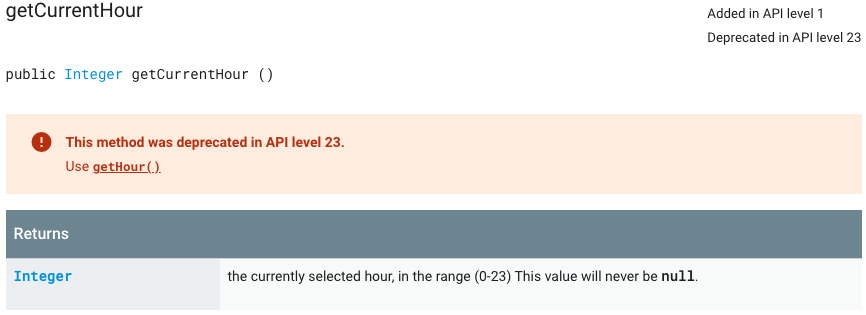
\includegraphics[width=0.8\linewidth]{deprecated-api-example.png}
%	\caption{An example of a deprecated API
%	}
%	\label{fig:deprecated_api_example}
%\end{figure*}

As an example, in Android API version 23, the method
\texttt{getCurrentHour()}, that had been present in the Android API since
version 1, was deprecated and the method \texttt{getHour()} was suggested
as its replacement.  Figure~\ref{fig:deprecated_api_update_example} shows
an example that modifies a usage of the method \texttt{getCurrentHour()} to
its replacement method \texttt{getHour()}. Given this example, one can
possibly learn a generic patch as shown in
Figure~\ref{fig:deprecated_api_update_edits}. The generic patch updates a
deprecated method usage to a replacement method usage.  Backward
compatibility is achieved by checking the version number of the mobile OS
running the app. If the version is greater than or equal to a certain
version number, the replacement method is used. Otherwise, the deprecated
method is used.

\begin{figure}[htb]
\centering
\begin{lstlisting}[language=diff,numbers=none]
private long addEventToGCal() {
  ...
  int hourInt;
  int minInt;
- hourInt = timepicker.getCurrentHour();
- minInt = timepicker.getCurrentMinute();
+ if (android.os.Build.VERSION.SDK_INT >=
+       android.os.Build.VERSION_CODES.M) {
+  hourInt = timepicker.getHour();
+  minInt = timepicker.getMinute();
+ } else {
+  hourInt = timepicker.getCurrentHour();
+  minInt = timepicker.getCurrentMinute();
+ }
  ...
}
\end{lstlisting}
\caption{A deprecated API-usage update}
\label{fig:deprecated_api_update_example}
\end{figure}

\begin{figure}[htb]
\centering
\begin{lstlisting}[language=diff,numbers=none]
- $T2 = $T1.getCurrentHour();
+ if (android.os.Build.VERSION.SDK_INT >=
+       android.os.Build.VERSION_CODES.M) {
+  $T2 = $T1.getHour();
+ } else {
+  $T2 = $T1.getCurrentHour();
+ }
\end{lstlisting}
\caption{A generic patch for updating uses of \texttt{getCurrentHour()}}
\label{fig:deprecated_api_update_edits}
\end{figure}

\jl{Figure \ref{fig:deprecated_api_update_edits} uses $-$ and $+$, but the
  AppEvolve paper uses I M D and U.  Furthermore, the figures in the
  AppEvolve paper don't use T1 and T2, and they don't use the syntax of
  real Java code.  Please don't just comment out this comment, but respond
  to it or do something about it.  It is important to represent AppEvolve
  accurately.}

\lx{Is this example intended to show the limitation of AppEvolve or a desired patch? This is related to the above sentence "..., one can possibly learn a generic patch as in Figure 2...": the sentence seems to imply the latter more; but if the example is more for showing the limitation of AppEvolve, it indeed should show the actual result from AppEvolve as accurately as possible and that sentence is better to be "..., AppEvolve would learn a patch as in Figure 2...". IMHO, it can be good to show both: first show the desired generic patch, and then show the actual patch from AppEvolve to show its limitations.}

\subsection{Approach}
\toolname\ takes as input a target app to update and a mapping from
deprecated API method(s) to the corresponding replacement API method(s).
Its processing is divided into four phases: {\em API-Usage Analysis}, {\em
  Update Example Search}, {\em Update Example Analysis} and {\em API-Usage
  Update}, as shown in Figure~\ref{fig:framework}.

In the {\em API-Usage Analysis} phase, \toolname\ accepts as input an {\em
  API Usage Change} and a {\em Target App}. An {\em API Usage Change}
describes the mapping from the deprecated API method(s) to the
corresponding replacement API method(s).  Information about this API usage
change may come, for example, from the documentation of the API itself. A
{\em Target App} is an app that contains a usage of the deprecated API
method and requires updates to make use of the replacement API
method. Given these two inputs, \toolname\ pinpoints the location of the
deprecated API usage in the target app. In the {\em Update Example
  Search} phase, \toolname\ searches GitHub for examples of API usage
updates that modify the usage of the deprecated API method to include the
usage of the replacement API methods. In the {\em Update Example Analysis}
phase, \toolname\ generates generic patches from the examples of API usage
updates and ranks these patches. In the {\em API Usage Update} phase,
\toolname\ tries to apply the ranked patches one by one and returns the
                 {\em Evolved Target App} if any of the edits is successful
                 and validated.

\begin{figure*}[t]
	\centering
	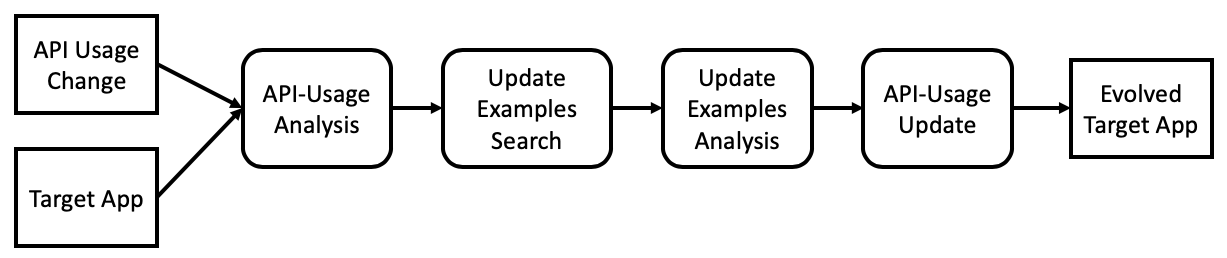
\includegraphics[width=0.8\linewidth]{framework.png}
	\caption{Framework of AppEvolve}
	\label{fig:framework}
\end{figure*}

We next describe each of the above phases in detail.
\subsubsection{API-Usage Analysis}
\toolname\ finds the location where the deprecated API method specified in
the {\em API Usage Change} is used inside the {\em Target App}. Consider
the deprecated API method \texttt{getCurrentHour()} mentioned in
Section~\ref{sec:problem}.  In this case, the {\em API Usage Change} is the
replacement of \texttt{getCurrentHour()} with \texttt{getHour()}. Given
this information, \toolname\ finds the location in the {\em Target App}
that invokes \texttt{getCurrentHour()}.

\subsubsection{Update Example Search}
\toolname\ searches for apps in GitHub that use both the deprecated and the
replacement API methods in their latest versions.  For each such app,
AppEvolve looks through the app history to find the commit where the uses
of the replacement API methods are added. This is intended to find examples
that produce a backward compatible Android app.  For each of these apps,
\toolname\ finds the changes that add the replacement API method to the app
code that already contains the deprecated API method. These changes are the
examples that can be used to update deprecated API method usages in other
apps.

\subsubsection{Update Example Analysis}
Given the examples found in GitHub, AppEvolve translates each example to a
generic patch. It does so by identifying edits related to the API usage via
intraprocedural forward and backward dependency analysis on the variables
involved in the API usage. Variables that are used in statements affected
by the edits but not defined by the edits themselves are considered as
context variables. All variables in the edits are then abstracted. Given
the generic patches, AppEvolve computes the common core of these generic
patches, defined as the longest subsequence of edits that are shared across
the patches. The generic patches are then ranked based on their distance to
the core.

\subsubsection{API-Usage Update}
Given a {\em Target App}, AppEvolve applies the generic patches according
to their rank computed in the previous phase. When applying a patch,
AppEvolve first finds mappings of the context variables to variables in the
{\em Target App}. For each such mapping, AppEvolve then tries to apply the
patch. If the edits are successfully applied, AppEvolve returns the {\em
  Evolved Target App}.

\subsection{Experiments}
For the target apps, the AppEvolve paper used 15 real-world apps from the
F-droid repository.\footnote{\url{https://fdroid.org}} These apps comprise
five apps for each of Android API versions 22, 23, and 25, and cover 20 API
usages in 41 locations. For each API version, the API change is manually
identified by reading the API documentation. Using the API change, the API
usage in each app is guaranteed to be: (1) different from the ones in the
other apps and (2) updated in the subsequent API version.  When applied to
the 15 apps considered, AppEvolve was able to update 17 out of 20 API
usages (85.00\% success rate) and 37 out of 41 (90.24\% success rate) of their occurrences across
the apps. %\jl{why no percentage?}



\section{Replication Settings}\label{sec:replication}
The goal of our replication study is to determine whether the observed
effectiveness of AppEvolve generalizes to a wider range of apps.

\subsection{Dataset}
Our replication study focuses on the same set of deprecated methods as the
original evaluation of AppEvolve and relies on the same training data, but
considers a larger set of mobile apps that use these deprecated methods.
We find the additional mobile apps by querying GitHub Code
Search\footnote{\url{https://github.com/search}} using the names of the
APIs. GitHub Code Search returns a list of ranked files matching the
query. Since Github Code Search only supports textual queries, it returns
many false positives, i.e., files that do not actually use the API methods
that were queried for.  Thus, we manually check that the considered files
contain the usages of the desired deprecated APIs.  We additionally check
that the considered files do not use the replacement APIs. Finally, we
randomly select 54 API usages, each from a different app in as our
dataset.  These usages are shown in Table~\ref{TODO}.

We note that although the AppEvolve training data also comes from GitHub,
there is no possible overlap with our dataset.  GitHub Code Search only
indexes the latest version of each repository.  The training data consists
of apps where the latest version uses the replacement API, while our test
data consists of apps that do not use the replacement API.  Thus, no
overlap is possible.

\subsection{Procedure}
For each app in our dataset, we must create an AppEvolve configuration. To
do so, we carefully read and understand the existing AppEvolve
configurations that were used in the original AppEvolve experiments. We
also asked the first author of AppEvolve to confirm how to configure
AppEvolve correctly. Finally, we ran our experiments in the virtual machine
environment provided by the AppEvolve
authors.\footnote{\url{https://sites.google.com/view/appevolve}}

After configuring AppEvolve for the apps, we ran AppEvolve on them. We
recorded the number of applicable and failed updates. We then categorized
the failed updates using card sorting\cite{...}. For this, we performed
multiple passes on the failed update data. In the first pass, we put each
of the failed updates into a category created based on our understanding of
the reason for the failure. In the subsequent passes, we reevaluated the
categories. We might rename a category to be more descriptive of the
problem that occurs in the set of updates belonging to the category, or
merge related categories into one. These steps were repeated until there
were no more changes to the categories.


\section{Findings}\label{sec:findings}
On our dataset, AppEvolve produces 10 applicable updates and 44 failed
updates. The original AppEvolve evaluation also showed 4 failed updates.
After investigating the 48 failed updates, we found some common reasons for
the failures, as described below. Table~\ref{table:data_statistic} shows
the number of occurrences of each of these issues.

% \begin{table}
% \caption{Update findings statistic}
% \begin{center}
% \begin{tabular}{ | p{8em} |c|c| } 
%  \hline
%  \textbf{Test Case Type} & \textbf{Detail of Cases} & \textbf{Number of Cases} \\ 
%  \hline
%  Work in AppEvolve & - & 10 \\ 
%  \hline
%  \multirow{7}{8em}{Fixed with simple refactor} & Total cases & 36 \\\cline{2-3} & Return statement & 6 \\\cline{2-3} & If statement & 1 \\\cline{2-3} & Method argument & 4 \\\cline{2-3} & Arithmetic operand & 3 \\\cline{2-3}  & Variable declaration & 12 \\\cline{2-3} & Complex expression & 20 \\\cline{2-3} 
%  \hline
%  \multirow{3}{8em}{Incomplete support of programming language features} & Inheritance & 2\\\cline{2-3} & Static modifier & 1 \\\cline{2-3} & Final modifier & 1\\\cline{2-3}
%  \hline
%  Unknown error & - & 4\\
%  \hline
% \end{tabular}
% \end{center}
% \label{table:data_statistic}
% \end{table}

\begin{table}
\caption{Update findings statistics}
\begin{center}
\begin{tabular}{ | p{12em} |c|c| } 
 \hline
 \textbf{Test Case Type} & \textbf{Subcategory} & \textbf{Occurrences} \\ 
 %\hline
 %Work in AppEvolve & - & 10 \\ 
 \hline
 \multirow{5}{12em}{Statements in the examples and at the target location are structurally different} & Return statement & 6 \\\cline{2-3} & If statement & 1 \\\cline{2-3} & Method argument & 4 \\\cline{2-3} & Arithmetic operand & 3 \\\cline{2-3}  & Declared variable & 12 \\\cline{2-3} 
 \hline
  \multirow{4}{12em}{Object and arguments of the deprecated API method are in the form of complex expressions} & - & 20\\&&\\&&\\&&\\
 \hline
 Edits beyond method boundaries & - & 3\\
\hline
 \multirow{3}{12em}{Incomplete support of programming-language features} & Inheritance & 2\\\cline{2-3} & Static modifier & 1 \\\cline{2-3} & Final modifier & 1\\\cline{2-3}
 \hline
 No examples & - & 1\\
 \hline
 Others & - & 4\\
 \hline
 \multicolumn{2}{|l|}{\bf Total} & 48\\
 \hline
\end{tabular}
\end{center}
\label{table:data_statistic}
\end{table}

\vspace{0.25\baselineskip}\noindent\textbf{1) The statements in the examples and at the target location are
 structurally different.} AppEvolve infers edit operations at the statement
 level (insert of a statement, move of a statement, etc).  Accordingly,
 AppEvolve is not able to apply changes inferred about method uses found
 in one kind of statement to a method use found in another kind of
 statement.  In the examples used in the evaluation of AppEvolve, it
 often occurs that the invocation of the deprecated API method
 is used as the right hand side of an assignment, while in our dataset the
 API method invocations occur in a variety of expression contexts.  We now
 present some examples:
\begin{itemize}
\item Return statement: 
In the code shown on the left side of Listing 1 in
Table~\ref{tab:mitigatesucc}, an invocation of the deprecated method {\tt
fromHtml} appears as part of a return statement of the {\tt getTitle}
method.

\item If statement test:
In the code shown on the left side of Listing 2 in
Table~\ref{tab:mitigatesucc}, an invocation of the deprecated method {\tt
requestAudioFocus} appears as a subexpression of the test expression of a
conditional.

\item Method argument:
In the code shown on the left side of Listing 3 in
Table~\ref{tab:mitigatesucc}, an invocation of the deprecated method {\tt
getCurrentHour} appears as the second argument of the method {\tt
String.format}.

\item Arithmetic operand:
In the code shown on the left side of Listing 4 in
Table~\ref{tab:mitigatesucc}, an invocation of the deprecated method {\tt
getCurrentHour} appears as the left argument of a concatenation with the
string {\tt ":"}.

\item Declared variable:
In the code shown on the left side of Listing 5 in
Table~\ref{tab:mitigatesucc}, an invocation of the deprecated method {\tt
getCurrentHour} appears as the initial value of a declared variable.  Even
though this case involves an assignment, such code does not match examples where
the assignment involves a previously declared variable.
\end{itemize}

\vspace{0.25\baselineskip}\noindent\textbf{2) Object and arguments of the
deprecated API method are in the form of complex expressions.} 
In creating edits, AppEvolve only abstracts over variables.  Accordingly,
when examples always contain variables for the object or the arguments, the
generated edits are not sufficient to update code in which these subterms
are expressed as more complex expressions.

In the code shown on the left side of Listing 5 in
Table~\ref{tab:mitigatesucc}, an invocation of the deprecated method {\tt
setTextAppearance} involves expressions that do not have the form
of a simple variable for both the object and arguments.

\vspace{0.25\baselineskip}\noindent\textbf{3) Edits beyond method boundaries.} AppEvolve cannot learn edits that modify program elements that reside outside of the method containing the API usage to be updated. These edits include operations such as adding imports and adding fields to a class. Below is a snippet of an update example that involves edits beyond method boundaries.
\begin{lstlisting}[language=diff,numbers=none]
18a19
+ import android.location.GnssStatus;
22a24
+ import android.os.Build;
33a36,37
+ private GnssStatus.Callback callback;
41c45,51
- locationManager.addGpsStatusListener(listener);
+ if (android.os.Build.VERSION.SDK_INT >= 
            android.os.Build.VERSION_CODES.N) {
+   locationManager.registerGnssStatusCallback(callback);
+ }
+ else{
+   locationManager.addGpsStatusListener(listener);
+ }
\end{lstlisting}
The above example involves a use of the deprecated API {\tt
addGpsStatusListener}. Updating a use of this API requires adding a private
field {\tt callback} of type {\em GnssStatus.Callback}.
since AppEvolve only learn edits inside a method containing the deprecated
API usage, it misses this necessary addition.

\vspace{0.25\baselineskip}\noindent\textbf{4) Incomplete support of programming language features.} AppEvolve fails to update cases in which the update involve programming language features such as:
\begin{itemize}
\item Inheritance: The code in the left hand side of Listing 7 in Table~\ref{tab:mitigatefail} shows an example of this case.  The deprecated API method is {\tt setAudioStreamType} of the class {\tt Media Player.} In the above snippet, {\tt TestMediaPlayer} extends {\tt MediaPlayer} and thus it inherits the {\tt setAudioStreamType} method. This method should be updated but AppEvolve does not seem to recognize it due to the use of inheritance.
\item Static modifier:  The code in the left hand side of Listing 8 in Table~\ref{tab:mitigatefail} shows an example of this case.  The deprecated API method {\tt requestAudioFocus} is invoked by {\tt mAudioManager}, which is a static field.

\item Final modifier: The code in the left hand side of Listing 9 in
Table~\ref{tab:mitigatefail} shows an example of this case.  Variable {\tt
paint} that is used as the fourth argument to the deprecated API method {\tt saveLayer} is a final field.

\end{itemize}

\vspace{0.25\baselineskip}\noindent\textbf{5) No examples.} No example for such API update that can be found in GitHub. 

\vspace{0.25\baselineskip}\noindent\textbf{6) Others.} These include cases that cannot be put to any category above.

\newcolumntype{Y}{>{\centering\arraybackslash}X}

\lstset{
	language=text,numbers=none,
	breaklines=true,
	aboveskip=-7pt,
	belowskip= -6pt
}

\begin{table*}
\centering
\caption{Successful simple refactoring mitigations that allows AppEvolve to generate applicable updates}\label{tab:mitigatesucc}
\begin{tabular}{|p{.10\textwidth}|p{.40\textwidth}|p{.40\textwidth}|}
\hline
\textbf{Listing}
  &
  \textbf{Original Code}
  &
  \textbf{Refactored Code}
 \\ \hline
1. Structurally different: return statement
&
\begin{lstlisting}
Spanned getTitle(){
    return Html.fromHtml(title);
}
\end{lstlisting}
&
\begin{lstlisting}[language=diff]
Spanned getTitle(){
+   Spanned a;
+   a = Html.fromHtml(title);
-   return Html.fromHtml(title);
+   return a;
}
\end{lstlisting}
\\ \hline
2. Structurally different: if statement
&
\begin{lstlisting}
public void play() {
    if (mAudioManager.requestAudioFocus(
    mAudioFocusListener, AudioManager.STREAM_MUSIC,
    AudioManager.AUDIOFOCUS_GAIN) != 
    AudioManager.AUDIOFOCUS_REQUEST_GRANTED) {
        return;
    }
}
\end{lstlisting}
&
\begin{lstlisting}[language=diff]
public void play() {
-   if (mAudioManager.requestAudioFocus
-     (mAudioFocusListener, AudioManager.
-           STREAM_MUSIC,
-     AudioManager.AUDIOFOCUS_GAIN) !=
-     AudioManager.AUDIOFOCUS_REQUEST_GRANTED) {
-     return;
-   }
+   int res;
+   int arg1=AudioManager.STREAM_MUSIC;
+   int arg2=AudioManager.AUDIOFOCUS_GAIN;
+   res = mAudioManager.requestAudioFocus (mAudioFocusListener, arg1, arg2);
+   if (res != AudioManager
+     .AUDIOFOCUS_REQUEST_GRANTED) {
+     return;
+   }
}
\end{lstlisting}
\\ \hline
3. Structurally different: method argument
&
\begin{lstlisting}
protected String getInputDataString() {
    return String.format("\%02d:\%02d", 
    timePicker.getCurrentHour(), 
    timePicker.getCurrentMinute());
}
\end{lstlisting}
&
\begin{lstlisting}[language=diff]
protected String getInputDataString() {
+   int hour;
+   hour = timePicker.getCurrentHour();
+   return String.format("%02d:%02d", hour,
+   timePicker.getCurrentMInute());
-   return String.format("\%02d:\%02d", 
-   timePicker.getCurrentHour(), 
-   timePicker.getCurrentMinute());
}
\end{lstlisting}
\\ \hline
4. Structurally different: arithmetic operand
&
\begin{lstlisting}
public void displayTime(View view) {
    String time = timePicker.getCurrentHour() 
	    + ":" + timePicker.getCurrentMinute();
    Toast.makeText(this, time, 
        Toast.LENGTH_SHORT).show();
}
\end{lstlisting}
&
\begin{lstlisting}[language=diff]
public void displayTime(View view) {
+   int hour;
+   hour = timePicker.getCurrentHour();
+   String time = hour + ":" +
+     timePicker.getCurrentMinute();
-   String time = timePicker.getCurrentHour()
-      + ":" + timePicker.getCurrentMinute();
    Toast.makeText(this, time, 
        Toast.LENGTH_SHORT).show();
}
\end{lstlisting}
\\ \hline
5. Direct assignment after declaration
&
\begin{lstlisting}
public Schedule generate() {
    TimePicker timePicker = (TimePicker) activity
        .findViewById(R.id.timePicker);
    int hours = timePicker.getCurrentHour();
    int minutes = timePicker.getCurrentMinute();
    SeekBar seekBar = (SeekBar) activity
        .findViewById(R.id.setLuminosity);
    int luminosity = seekBar.getProgress();
    return new Schedule(hours, minutes, luminosity);
}
\end{lstlisting}
&
\begin{lstlisting}[language=diff]
public Schedule generate() {
    TimePicker timePicker = (TimePicker) activity
        .findViewById(R.id.timePicker);
+   int hours;
+   hours = timePicker.getCurrentHour();
-   int hours = timePicker.getCurrentHour();
    int minutes = timePicker.getCurrentMinute();
    SeekBar seekBar = (SeekBar) activity
        .findViewById(R.id.setLuminosity);
    int luminosity = seekBar.getProgress();
    return new Schedule(hours, minutes, luminosity);
}
\end{lstlisting}
\\ \hline
6. Complex expressions
&
\begin{lstlisting}
protected void onClick() {
    ...
    Dialog d = builder.create();
    d.show();
    ((TextView) d.findViewById(android.R.id.message))
        .setTextAppearance(getContext(), 
        android.R.style.TextAppearance_Small);
    ...
}
\end{lstlisting}
&
\begin{lstlisting}[language=diff]
protected void onClick() {  
    ...
    Dialog d = builder.create();
    d.show();
-   ((TextView) d.findViewById(android.R.id.
-     message))
-   .setTextAppearance(getContext(), 
-    android.R.style.TextAppearance_Small);
+   Context c = getContext();
+   int i = android.R.style.
+         TextAppearance_Small;
+   TextView t = ((TextView) d.findViewById
+     (android.R.id.message)); 
+   t.setTextAppearance(c, i);
    ...
}
\end{lstlisting}
\\ \hline


\end{tabular} 
\end{table*}

\begin{table}
	\caption{Failed categories that are unhandled by our mitigations}\label{tab:mitigatefail}
\centering
\begin{tabular}{|p{.08\textwidth}|p{.35\textwidth}|}
\hline
\textbf{Listing}
  &
  \textbf{Original Code}
 \\ \hline
7. Incomplete support: inheritance
&
\begin{lstlisting}
public class TestMediaPlayer extends MediaPlayer {
    public TestMediaPlayer() {
        setAudioStreamType(AudioManager.STREAM_MUSIC);
    }
    public TestMediaPlayer(Context testContext, 
        int withResource) throws Exception {
        this();
        AssetFileDescriptor afd = 
            testContext.getResources()
            .openRawResourceFd(withResource);
        assertNotNull(afd);
        setDataSource(afd.getFileDescriptor()
            , afd.getStartOffset(), afd.getLength());
        afd.close();
        prepare();
    }
}
\end{lstlisting}
\\ \hline
8. Incomplete support: static
&
\begin{lstlisting}
private static AudioManager mAudioManager;
private static OnAudioFocusChangeListener afChangeListener;
public static void requestAudioFocus
    (Context context) {
    if(mAudioManager == null){
        mAudioManager = (AudioManager) 
            context.getApplicationContext()
            .getSystemService
            (Context.AUDIO_SERVICE);
    }
    mAudioManager.requestAudioFocus(
        afChangeListener,
        AudioManager.STREAM_MUSIC,
        AudioManager.AUDIOFOCUS_GAIN);
}
\end{lstlisting}
\\ \hline
9. Incomplete support: final
&
\begin{lstlisting}
private final Paint paint;
@Override protected void onDraw(Canvas canvas) {
    super.onDraw(canvas);
    canvas.drawColor(Color.GREEN);
    canvas.saveLayer(0, 0, canvas.getWidth(),
        canvas.getHeight(), paint, 
        Canvas.ALL_SAVE_FLAG);
    canvas.restore();
}
\end{lstlisting}
\\ \hline
 \end{tabular}
 \end{table}

  \lstdefinelanguage{text}{
	basicstyle=\ttfamily\extrabold\scriptsize,
	identifierstyle=\color{black},
	aboveskip=5pt,
	belowskip= 5pt
}


\section{Mitigations}\label{sec:mitigations}
To mitigate the observed failures, we tried to modify the deprecated API
usages in the target app's source code so that AppEvolve could produce an
applicable update. Looking at the 10 apps that were updated successfully,
we observe that in each case the invocation of the deprecated method
appears as the right hand side of an assignment statement, or any
arguments of the deprecated method are simple variables.
We transform the remaining apps where possible accordingly, converting the
invocations of the deprecated APIs to a form reminiscent of the three
address code used in compiler intermediate representations \cite{dragon}.
The right side of Table~\ref{tab:mitigatesucc} shows a diff that applies
these mitigations on the cases presented in Section~\ref{sec:findings}
where the mitigation allows AppEvolve to produce applicable updates.

\begin{enumerate}
\item After the refactoring described in Listing 1
Table~\ref{tab:mitigatesucc}, rather than directly returning the result of
invoking the deprecated method {\tt fromHtml}, we first assign it to a fresh
variable named {\tt a} of type {\tt Spanned}.

\item After the refactoring described in Listing 2 of
Table~\ref{tab:mitigatesucc}, rather than directly inserting the constants
{\tt AudioManager.STREAM\_MUSIC} and {\tt AudioManager.AUDIOFOCUS\_GAIN} as
the second and third arguments of {\tt requestAudioFocus}, we first assign
them to fresh {\tt int}-typed variables {\tt arg1} and {\tt arg2},
respectively. Moreover, the result of invoking {\tt requestAudioFocus} is
assigned to a fresh variable named {\tt res} of type {\tt AudioManager}
that is then used in the if condition.

\item After the refactoring described in Listing 3 of
Table~\ref{tab:mitigatesucc}, rather than directly inserting the result of
invoking {\tt getCurrentHour} as the second argument of {\tt
String.format}, the result is first assigned to fresh a variable named {\tt hour}
of type {\tt int}.

\item After the refactoring described in Listing 4 of
Table~\ref{tab:mitigatesucc}, rather than concatenating the result of {\tt
getCurrentHour} directly to ``:'', the result is first assigned to a fresh
variable named {\tt hour} of type {\tt int}.

\item After the refactoring described in Listing 5 of
Table~\ref{tab:mitigatesucc}, rather than directly assigning the result of
invoking {\tt getCurrentHour} to the variable {\tt hours} when it is
declared, we declare {\tt hours} first and then assign the result of
invoking {\tt getCurrentHour} to {\tt hours}.

\item After the refactoring described in Listing 6 of
Table~\ref{tab:mitigatesucc}, rather than invoking {\tt setTextAppearance}
directly from the object returned by invoking {\tt findViewById}, the
returned object is first assigned to a variable named {\tt t} of type {\tt
TextView}. {\tt setTextAppearance} is then invoked from {\tt t}.

\end{enumerate}

In essence, our mitigations refactor the deprecated method invocation in
the target app to resemble the examples from which AppEvolve learns
edits. Our mitigations result in 38 successful updates out of the 44 failed
updates on the apps in our dataset (86\% success rate).


\section{Discussion}\label{sec:discuss}
In this section, we discuss some threats to validity, the relation of our
results to those originally presented for AppEvolve, cases that are not
handled by our mitigations, and future directions for improving the
approach to updating deprecated API usage in Android apps.

\subsection{Threats to Validity}

One threat is related to whether we have configured AppEvolve correctly. To
mitigate this threat, we have tried our best to run AppEvolve following the
instructions given by the authors in the AppEvolve documentation. We have
also asked AppEvolve's first author how to configure AppEvolve correctly
for new mobile apps. Based on the information obtained, we independently
reconstructed the configurations for the target apps in the original
dataset, and using these configurations were able to reproduce the results
reported for that dataset.  We have also rechecked our configurations for
the new dataset several times. We have released a replication package for
others to check and
validate.\footnote{\url{https://sites.google.com/smu.edu.sg/appevolve-replication}}

Another threat is related to the generalizability of the findings. We have added 54 new applications to evaluate the effectiveness of
AppEvolve in generating applicable updates. This translates to 54 API usage
locations on top of the 41 API usage locations in AppEvolve dataset, thus
more than doubling the number of API usage locations and more than tripling the number of apps as compared to the dataset used in the original work. We
believe this is sufficient to understand the capabilities of AppEvolve, as
44 of the 54 API usages that we have added uncover limitations of
AppEvolve. There might be other cases that AppEvolve cannot handle, but we
believe that we have found many of them.

\subsection{Cases Not Handled by Our Mitigation Strategy}

There are 8 failed updates in our dataset where our mitigation
strategy is not successful. For the cases of {\tt static} and {\tt final}
annotations, representing two failed updates where our mitigations do not
work, we manage to manually alter the target code such that AppEvolve can
successfully apply the learned edits. We present these cases below.

We modified the code on the left side of Listing 8 in
Table~\ref{tab:mitigatefail} following the diff shown below. In the
original code, a static field {\tt afChangeListener} of type {\tt
  Audio\-Manager.OnAudioFocusChangeListener} is directly put as the first
argument of {\tt requestAudioFocus} and AppEvolve cannot generate an
applicable update. When {\tt afChangeListener} is assigned to a local
variable named {\tt af} in addition to our mitigation, AppEvolve can
generate an applicable update.

%\vspace{\baselineskip}

\begin{lstlisting}[language=diff,numbers=none]
private static AudioManager mAudioManager;
private static OnAudioFocusChangeListener afChangeListener;
public static void requestAudioFocus
    (Context context) {
    if(mAudioManager == null){
        mAudioManager = (AudioManager) context
            .getApplicationContext()
            .getSystemService(Context.AUDIO_SERVICE);
    }
-   mAudioManager.requestAudioFocus(
-       afChangeListener,
-       AudioManager.STREAM_MUSIC,
-       AudioManager.AUDIOFOCUS_GAI
+   int res;
+   int a = AudioManager.STREAM_MUSIC;
+   int b = AudioManager.AUDIOFOCUS_GAIN;
+   AudioManager am = mAudioManager;
+   AudioManager.OnAudioFocusChangeListener
+        af = afChangeListener;
+    res = am.requestAudioFocus(af,a,b);
}
\end{lstlisting}

\vspace{\baselineskip}

We modified the code on the left side of Listing 9 in
Table~\ref{tab:mitigatefail} following the diff shown below.

%\vspace{\baselineskip}

\begin{lstlisting}[language=diff,numbers=none]
-private final Paint paint;
+private Paint paint;
@Override protected void onDraw(Canvas canvas) {
    super.onDraw(canvas);
    canvas.drawColor(Color.GREEN);
+   float a = 0;
+   float b = 0;
+   float c = getWidth();
+   float d = getHeight();
+   int flag = Canvas.CLIP_SAVE_FLAG;
+   canvas.saveLayer(a,b,c,d, paint, flag);
-   canvas.saveLayer(0, 0, canvas.getWidth(),
-       canvas.getHeight(), paint,
-       Canvas.ALL_SAVE_FLAG);
    canvas.restore();
  }
\end{lstlisting}

\vspace{\baselineskip}

In the original code, the field named {\tt paint} of type {\tt Paint} has a
{\tt final} modifier. Removing this modifier after performing our
mitigation results in an applicable update. It suggests that AppEvolve does
not support the {\tt final} modifier.

\subsection{Result assessment}

We were initially surprised by the large difference between the results on
our data set, where we obtained a success rate of 18.51\%, and the results
reported by the authors of AppEvolve, who obtained a success rate of
85.00\%, even though our dataset was constructed randomly, without taking
into account the strengths or weaknesses of AppEvolve.  Indeed, given that
AppEvolve relies on matching statements, abstracting only over variables,
it is surprising that AppEvolve could achieve such high accuracy on
e.g.\ simple getter methods such as {\tt getCurrentHour()} (e.g., Listing
3). In our dataset, such methods are often used as subexpressions of
arbitrarily complex statements, which may contain project-specific code.
Likewise, as illustrated by Listing 2, invocations of method calls may have
arbitrarily complex, possibly project-specific, arguments that are not
likely to be found in other codebases.

To understand better how AppEvolve is able to achieve a high rate of
success in the previously reported evaluation, we investigate the examples
and target apps used.  Given the difficulty of finding the original files
for the examples, for which no origin information is provided, we focus on
a single example, the call to {\tt getCurrentHour()} in the app {\sc
  Conversations} version 1.8.0 in F-Droid (A02-U03 in the AppEvolve paper).
In F-Droid, we find that the only invocation of {\tt getCurrentHour()}
occurs in the argument list of a call to the {\tt set} method of the {\tt
  Calendar} class, a code structure similar to the code shown on the left
side of Listing 3.  In the AppEvolve dataset, this call is extracted into a
separate statement, analogous to our mitigation shown on the right side of
Listing 3.  We have furthermore looked at one of the examples provided for
this API, and have found the original code on GitHub in the file {\tt
  RepeaterDialogFragment.java} from the {\tt
  marekpiotrowskimp/nyndro\_remote} repository.  Again, we find that in the
GitHub code, the call appears in an argument list, while the corresponding
example in the AppEvolve example set has been transformed analogous to our
mitigation.  These changes convert invocations that occur in differing
contexts to invocations that can be exploited by AppEvolve.

We note that the observed issue appears to be a direct result of the key
design decision of AppEvolve, of not merging examples.  Merging could
motivate discarding irrelevant context of the use of the deprecated method
and extending the abstraction of subterms beyond variables, but, as observed
by the authors of AppEvolve, it could discard some information
that is necessary to correctly perform the transformation.

\subsection{Future Directions}

Our above analysis suggests that our mitigation succeeds because the
AppEvolve authors have already performed such a mitigation in the change
examples included in the AppEvolve replication package.  To improve the
results of AppEvolve in the more general case, a solution could be to
systematically first normalize the change examples to a standard form.
Edits can then be learned from this standard form. When the edit is applied
to a new piece of code, that target code should also be normalized, to
minimize the code variations. If the edits are successfully applied, the
resulting code can then be refactored again to restore the coding style of
the developers.  Our mitigations represent a subset of the normalizations
that may be possible.

Any tool that automatically transforms code runs the risk of converting the
code to a style that is incompatible with the preferences of the given
app's developers.  In the case of AppEvolve, there is already the risk of
changing the existing coding style to the coding style found in the app
providing the change example, and any normalization performed to the target
code further increases this risk.  To assess the impact of AppEvolve on
coding style, we perform a simple experiment to compare the output of
AppEvolve after applying our mitigation with code that is manually updated
to deal with a set of deprecated APIs.  We asked a software engineer who is
not an author of this paper to update the code shown on the left hand side
of Listing 4 in Table~\ref{tab:mitigatesucc}. The code generated by
AppEvolve and by the engineer is shown below.

%Buse and Weimer~\cite{Buse:2008:MSR:1390630.1390647} propose a metric of
%software readability that are based on a set of simple local features. They
%also provide an automatic readability measure model that is built on 12,000
%code readability judgments. We run this model and compare the readability
%measure of the API update created by AppEvolve against that of the update
%created by the human.  Scores range from 0 to 1 where, 0 is least and 1 is
%most readable.

\vspace{0.2cm}\noindent {\bf AppEvolve's Update}\ft{Need to update this example}
\begin{lstlisting}[language=diff,numbers=none]
public void displayTime(View view){
  int varInt1;
  int varInt2;
  if (android.os.Build.VERSION.SDK_INT >=
      android.os.Build.VERSION_CODES.M) {
    varInt1=timePicker.getHour();
  }
  else {
    varInt1=timePicker.getCurrentHour();
  }
  if (android.os.Build.VERSION.SDK_INT >=
      android.os.Build.VERSION_CODES.M) {
    varInt2=timePicker.getMinute();
  }
  else {
    varInt2=timePicker.getCurrentMinute();
  }
  String time=varInt1 + ":" + varInt2;
  Toast.makeText(this,time,Toast.LENGTH_SHORT).show();
}
\end{lstlisting}


\vspace{0.2cm}\noindent {\bf Engineer's Update}
\begin{lstlisting}[language=diff,numbers=none]
public void displayTime(View view) {
    String time;
    if (android.os.Build.VERSION.SDK_INT >= 23) {
        // only for gingerbread and newer versions
        time = timePicker.getHour() + ":" +
               timePicker.getMinute();
    } else {
        time = timePicker.getCurrentHour() + ":" +
               timePicker.getCurrentMinute();
    }
    Toast.makeText(this, time, Toast.LENGTH_SHORT).show();
}
\end{lstlisting}

%\jl{the following two paragraphs have to be merged.}

\vspace{0.5cm}The code made manually by the engineer is substantially
different from the code produced by AppEvolve, and developers may indeed
prefer the code made by the engineer. In particular, the engineer did not
introduce fresh variables and introduced only one test of the Android
version, covering both method uses.  Future work may investigate how to
restore the original coding style after applying AppEvolve. One step would
be to choose good names for the newly introduced variables. Some recent
studies use deep learning and mining software repositories to recommend
method and class names~\cite{allamanis2015suggesting}. These approaches can
potentially be extended for inferring good variable names in our context.


\section{Related Work}\label{sec:related}
%In this section, we present prior works on API deprecation, API evolution, and API migration.
\subsection{API Deprecation}
There are a lot of works that focus on studying API deprecation~\cite{zhou2016api,kapur2010refactoring,raemaekers2014semantic,brito2016developers,robbes2012developers,sawant2016reaction,sawant2018features,li2018characterising}. Zhou and Walker~\cite{zhou2016api} found that, in practice, deprecating APIs does not always follow {\em deprecated-replace-remove} cycle, such as many deprecated APIs are undeprecated. They also developed a tool to warn about deprecated API usages in StackOverflow posts. Kapur et al.~\cite{kapur2010refactoring} found that APIs might be removed without being marked as deprecated. Raemaekers et al.~\cite{raemaekers2014semantic} discovered that some Java artifacts on the Maven Central Repository never remove deprecated APIs. Brito et al.~\cite{brito2016developers} showed that not all APIs are annotated with replacement messages. Robbes et al.~\cite{robbes2012developers} analyzed the Smalltalk ecosystem and showed that some API changes caused by deprecation can substantially impact the ecosystem. This study was replicated on the Java ecosystem and similar results were reported~\cite{sawant2016reaction,sawant2018reaction}, except that the number of deprecated API replacements was higher in the Smalltalk ecosystem. Sawant et al.~\cite{sawant2018features} created a taxonomy containing 12 reasons for deprecation and developed an approach to automatically classify them. Li et al.~\cite{li2018characterising} performed an exploratory study on characterizing Android APIs. They found that, among other things, deprecated Android APIs are not always consistently annotated and documented, and they are also regularly cleaned up. They have also developed a prototype tool that can generate API replacement mappings from the Android framework source code. %However, the automatically generated mappings may not be correct. In contrast, we have manually curated our dataset of 647 deprecated method mappings.
%\lx{"these mappings"? It sounds like the mappings auto-generated by Li et al. are correct? May be better to give some numbers to show how our curated dataset is different from their mappings.}

All of the above studies aim to understand API deprecation. In this work,
we aim to understand the applicability of a state-of-the-art approach for
automatic update of Android apps, which updates uses of deprecated methods to
corresponding uses of their replacement methods.

%% \subsection{API Evolution}

%% There are many works that focus on supporting API
%% evolution~\cite{henkel2005catchup,schafer2008mining,wu2010aura,dagenais2009semdiff,dagenais2011recommending,meng2012history,yu2017api}. Henkel
%% et al.~\cite{henkel2005catchup} created a tool named CatchUp! that records
%% developers' refactoring actions when evolving uses of an API within an
%% Integrated Development Editor (IDE) and can replay them afterwards. Xing et
%% al.~\cite{xing2007api} proposed Diff-CatchUp!, a tool that recommends
%% plausible replacements for obsolete API usages following example changes in
%% the API change history.  Sch{\"a}fer et al.~\cite{schafer2008mining}
%% proposed to mine API replacement rules for API evolution by analyzing
%% client code that has performed the replacements. Dagenais and
%% Robillard~\cite{dagenais2009semdiff,dagenais2011recommending} proposed an
%% approach named SemDiff that learns how an API adapts to its own changes and
%% uses this information to recommend a set of method replacements to client
%% programs. Wu et al.~\cite{wu2010aura} developed a tool named AURA to mine
%% API replacement rules using a combination of method call dependency
%% analysis and text similarity. Meng et al.~\cite{meng2012history} proposed
%% HiMA, a tool that infers API replacement rules between two versions of a
%% framework by aggregating API replacement rules for each pair of consecutive
%% revisions in the framework history between the two versions. Yu et
%% al.~\cite{yu2017api} develop an approach named AUC-Miner, which mines API
%% replacement rules by employing context information to refine method call
%% dependency analysis.

%% %In this work, given the API replacement rules, our approach generates transformation rules, in the form of semantic patches, that can be used to perform the API replacement. Thus, our approach complements approaches that mine API replacement rules.

%% \subsection{API Migration}

%% Many works have been proposed to support API migration in varying
%% situations~\cite{hora2015apiwave,zhou2016api,nguyen2010graph,nguyen2014statistical,nita2010using,lamothe2018a4}. Nita
%% and Notkin~\cite{nita2010using} proposed the use of twinning (i.e., a
%% technique to specify program changes without modifying the program
%% directly) to migrate a program to use alternative APIs. Hora and
%% Valente~\cite{hora2015apiwave} proposed Apiwave, a tool for tracking API
%% popularity and migration. Zhong et al.~\cite{zhou2016api} developed a tool
%% called MAM, which mines API mappings for language migration from programs
%% with two versions in two programming languages. Nguyen et
%% al.~\cite{nguyen2010graph} developed LIBSYNC, which employs a graph based
%% approach to migrate API usage in client code to the new version of the API
%% by learning from clients that have performed the adaptations. Nguyen et
%% al.~\cite{nguyen2014statistical} proposed StaMiner, a statistical model
%% based approach to mine API mappings for migrating programs from one
%% language to another. Lamonthe et al.~\cite{lamothe2018a4} proposed an
%% approach that learns API migration patterns from code examples and can
%% apply these patterns to migrate deprecated APIs.

\subsection{Program Transformation}
Research on program transformation have been done in multiple works~\cite{Visser:2001:SLP:647200.718711, Meng:2013:LLA:2486788.2486855, Rolim:2017:LSP:3097368.3097417,Long:2017:AIC:3106237.3106253, Bavishi:2019:PAD:3338906.3338952, Andersen:2012:SPI:2351676.2351753}. Visser~\cite{Visser:2001:SLP:647200.718711, 10.1007/978-3-540-87875-9_13, Lee:2013:DRI:2486788.2486792, Nguyen:2019:GMI:3339505.3339608} proposed Stratego, a language for program transformation that is based on rewriting strategies. Stratego aims to make reusable transformation rules that can be used in multiple transformations by separating the strategies from the transformation rules. Meng et al.~\cite{Meng:2013:LLA:2486788.2486855} developed LASE, a tool that can create edit script from examples, locate the edit locations, and do the code transformation automatically. Rolim et al.~\cite{Rolim:2017:LSP:3097368.3097417} proposed REFAZER, a technique for automatic program transformation generation which is build based on code edits performed by developers as input-output examples. Long et al.~\cite{Long:2017:AIC:3106237.3106253} proposed Genesis which can automatically infer patch generation transforms from previous successful patches. Bavishi et al.~\cite{Bavishi:2019:PAD:3338906.3338952} developed PHOENIX, a fully automated pipeline system that mines and clean patches from examples and learns generalized executable repair strategies by leveraging a novel Domain Specific Language (DSL). Andersen et al.~\cite{Andersen:2012:SPI:2351676.2351753} proposed the tool spdiff that can infer transformation specifications from examples of both original and updated code. Robbes and Lanza~\cite{10.1007/978-3-540-87875-9_13} presented a system that support example-based program transformation. The system takes an example manual change by developer and generalizes it to other application contexts. Lee et al.~\cite{Lee:2013:DRI:2486788.2486792} implemented DNDRefactoring, a tool that streamline the configuration and invocation of refactoring system through the use of direct manipulation via drag-and-drop. Nguyen et al.~\cite{Nguyen:2019:GMI:3339505.3339608} proposed a graph-based mining approach on detecting repetitive code changes called as CPatMiner. This approach aims to detect semantic code change patterns from large corpus and present them as graph.

\subsection{Replication Studies}

There have been a number of replication studies in the software engineering
domain \cite{Chen:2017:CLP:3042021.3042046,
  Greiler:2015:COS:2820518.2820522, Akbarinasaji:2018:PBT:3174380.3174639,
  Dinh-Trong:2005:FPR:1079843.1080069, howdopython} that have not always
confirmed the original results. Chen and
Jiang~\cite{Chen:2017:CLP:3042021.3042046} replicated a study by Yuan et
al.~\cite{Yuan:2012:CLP:2337223.2337236} of logging practices.  In contrast
to the observations of Yuan et al., Chen and Jiang found that bug reports
without a log message take a shorter time to resolve than bug reports that
include a log.  Greiler et al.~\cite{Greiler:2015:COS:2820518.2820522}
replicated the work of Bird et al.~\cite{Bird:2011:DTM:2025113.2025119} on
the correlation between code ownership and software quality.  Greiler et
al. used new and refined code ownership metrics and prediction
models. Akbarinasaji et al.~\cite{Akbarinasaji:2018:PBT:3174380.3174639}
replicated and reinforced the finding on the bug fixing time estimation
model by showing similar result with the previous work. A replication study
on open source development by Trong et
al.~\cite{Dinh-Trong:2005:FPR:1079843.1080069} found new findings from the
previous work by Mockus et al.~\cite{Mockus:2002:TCS:567793.567795}. They
supported some of the previous hypotheses and proposed revisions on hypothesis related to the need of formal arrangement for work coordination and on hypothesis regarding the number of core developers on open source project. A
replication study by Orru et al.~\cite{howdopython} conducted an analysis
of the use of inheritance in Python systems that was previously done on
Java. Their result shows that compared on the previous findings on Java,
Python has more classes that are inherited from but fewer classes that inherit from other
classes.

%Among the API migration work above, Lamonthe et al.'s work is the closest to our work. Our work also deals with API migration, particularly replacing deprecated APIs. However, different than their work, our work focuses on the scenario in which there are no examples. 

% \subsection{API Usage Recommendation}
% Several approaches have been developed to recommend and explore how an API can be used~\cite{glassman2018visualizing}. Glassman et al.~\cite{glassman2018visualizing} proposed EXAMPLORE, an tool that summarizes hundreds of code examples for an API in a single view.


\section{Conclusion and Future Work}\label{sec:conclusion}
AppEvolve is the state-of-the-art approach for automatic update of
deprecated-API usage in Android apps. Experiments previously reported for
AppEvolve have shown that it can generate applicable updates for
85.00\% of these API
changes and 90.24\% of their usage locations on mobile apps in the
AppEvolve dataset.

In this work, we evaluate whether this observed effectiveness is
generalizable. We add 54 additional mobile apps that use the APIs contained
in the AppEvolve dataset. Running AppEvolve on these mobile apps shows that
AppEvolve fails to generate applicable updates for 81.48\% of the mobile
apps. By analyzing these failed cases, we found that they failed mainly
due to:
\begin{enumerate}
    \item Statements in the examples and at the target location are structurally different.
    \item Object and arguments of the deprecated API method are in the form of complex expressions.
    \item Edits are required beyond method boundaries.
    \item Incomplete support of programming language features.
    \item No examples found in GitHub.
\end{enumerate}
We mitigate the first and the second categories by performing a simple
refactoring that modifies the code containing API usage in the target app
to resemble the one in the example. Our mitigations enable AppEvolve
to generate applicable updates for 81.82\% of the failed cases.

To try to resolve the discrepancy in the findings, we looked closer at the
examples and target apps used by finding the original examples and target
apps. We found that they were transformed analogous to our mitigation.
These transformations convert invocations in various contexts into code
exploitable by AppEvolve.

Based on our findings, we propose future directions for automatic update of
deprecated-API usage in Android apps, which include code normalization to
ensure that both the example of API usage and the target app code are in
the same standard form to minimize the variety of ways that the code is
written. Using this technique, simple refactoring that we use to mitigate
the failed cases may not be necessary. We also propose the usage of
identifier name recommendation to name new variables that may have been
introduced due to code normalization.



\balance

\bibliography{references}
\bibliographystyle{plain}

\end{document}
